%        File: DesignDocument.tex
%     Created: 一 3月 26 01:00 下午 2018 C
% Last Change: 一 3月 26 01:00 下午 2018 C
%
\documentclass[UTF8,noindent]{ctexart}
\usepackage[a4paper,left=2.0cm,right=2.0cm,top=2.0cm,bottom=2.0cm]{geometry}
\usepackage{hyperref}
\usepackage{url}
\usepackage{graphicx}
\usepackage{amsmath}
\usepackage{amssymb}
\usepackage{enumitem}
\usepackage{tikz}
\usepackage{float}
\usepackage{xeCJK}
\usepackage{listings}
\usepackage{xcolor}
\lstset{language = c,numbers=left, showstringspaces=false,keywordstyle= \color{ blue!70 },commentstyle=\color{red!50!green!50!blue!50}, frame=shadowbox, rulesepcolor= \color{ red!20!green!20!blue!20 } 
} 
\CTEXsetup[format={\Large\bfseries}]{section}
\usetikzlibrary{graphs}
\title{\CJKfamily{zhkai}计算机网络研讨课实验报告}
\author{{\CJKfamily{zhkai}冯吕}\ $2015K8009929049$}
\date{\today}
\begin{document}
\maketitle
\zihao{5}
\CJKfamily{zhsong}
%\begin{center}
%  \begin{tabular}{|p{15cm}|}
%    \hline
\section*{{\CJKfamily{zhhei}实验题目}}$Socket$ 应用编程实验
%\hline
\section*{{\CJKfamily{zhhei}实验内容}}在本次实验中,需要实现一个基于$Socket$的字符统计程序。

首先,有两个文件,$workers.conf$配置文件中存储了所有$worker$的$IP$,$war\_and\_peace.txt$文件则是需要统计字符的文件。因此,在本次实验中,需要分别实现$master$和$worker$,首先,$master$需要读取$worker$的配置文件,即获得$worker$的$IP$,然后与$worker$建立连接,连接成功之后,将任务分发给各个$worker$,$worker$接收到消息后,进行字符统计,然后把统计结果返回给$master$,然后$master$整合统计结果并将结果输出到屏幕上。\\
		%\hline
		\section*{{\CJKfamily{zhhei}实验流程}}
		本次实验需要实现对应的$master$和$worker$,对应的源程序为$master.c$和$worker.c$,它们所实现的功能如下:

		\begin{enumerate}
		\item $master$读取配置文件,获取$IP$,$IP$数为$2$,因此,建立两个$Socket$,分别与一个$worker$建立连接。
\begin{lstlisting}
// Create socket
if ((s1 = socket(AF_INET, SOCK_STREAM, 0)) < 0) {
    perror("Could not create socket\n");
    return -1;
		}
if ((s2 = socket(AF_INET, SOCK_STREAM, 0)) < 0) {
    perror("Could not create socket\n");
    return -1;
}
printf("Socket created\n");

// Read workers' conf
FILE *fp;
if ( !(fp = fopen("./workers.conf", "r")) ){
	printf ( "Open config file failed!\n" );
	return 1;
}
if (!(fgets(ip1, bufferSize, fp) && fgets(ip2, bufferSize, fp))){
	printf ( "Read config file failed!\n" );
	return 0;
}
fclose(fp);
struct sockaddr_in worker1, worker2;

worker1.sin_addr.s_addr = inet_addr(ip1);
worker1.sin_family = AF_INET;
worker1.sin_port = htons(8888);
worker2.sin_addr.s_addr = inet_addr(ip2);
worker2.sin_family = AF_INET;
worker2.sin_port = htons(8888);

// connect to worker
if (connect(s1, (struct sockaddr *)&worker1, sizeof(worker1))<0){
	perror( "Connect worker1 failed!\n" );
	return 1;
}
if (connect(s2, (struct sockaddr *)&worker2, sizeof(worker2))<0){
	perror( "Connect worker2 failed!\n" );
	return 1;
}
printf ("Connected all workers!\n");
\end{lstlisting}

\item 对于每个$worker$来说,首先创建一个$Socket$,然后进行绑定,绑定完成之后,等待着$master$来连接。
\begin{lstlisting}
sock = socket(AF_INET, SOCK_STREAM, 0);
if (sock == -1) {
	printf("Could not create socket\n");
}
printf("Socket created\n");

// Prepare the sockaddr_in structure
worker.sin_family = AF_INET;
worker.sin_addr.s_addr = INADDR_ANY;
worker.sin_port = htons(8888);

if ( bind(sock, (struct sockaddr *)&worker, sizeof(worker)) <0 ){
	perror( "bind failed. Error\n" );
	return -1;
}

//waiting for master to connect
listen(sock, 3);
printf ( "Waiting for incoming connectionos...\n" );
\end{lstlisting}

\item $master$与两个$worker$建立连接之后,需要分发任务。首先,通过文件操作获取文件中的总字符数目,然后将前一半分给第一个$worker$统计,后一半分给另一个。因此,发送给$worker$的消息总共占$30$个字节,四个字节为字节数,四个字节为$worker$需要统计的起始位置,四个字节为终止位置,剩余的十八个字节为文件名(包括字符串中的最后一个空字符)。
\begin{lstlisting}
// open count file
int numOfChar = 0;
FILE *fpc;
if ( !(fpc = fopen("./war_and_peace.txt", "r")) ){
	printf ( "Open war_and_peace.txt failed!\n" );
	return 1;
}
//count all char nums
while( (fgetc(fpc)) != EOF ){
	++numOfChar;
}
fclose(fpc);
int middle = numOfChar / 2;
int total = 30;
int zero = 0;

char loc[] = {'w', 'a','r','_','a','n','d',
    '_','p','e','a','c','e','.','t','x','t','\0'};
void *message1 = malloc (30);
void *message2 = malloc (30);
memcpy((void *)message1, &total, 4);
memcpy((void *)((int *)(message1) + 1), &zero, 4);
memcpy((void *)((int *)(message1) + 2), &middle, 4);
strncpy(((char *)message1 + 12), loc, 18);
memcpy((void *)message2, &total, 4);
memcpy((void *)((int *)(message2) + 1), &middle, 4);
memcpy((void *)((int *)(message2) + 2), &numOfChar, 4);
strncpy(((char *)message2 + 12), loc, 18);

//send work to workers
if ( send(s1, message1, 30, 0) < 0 ){
	printf ( "Send to worker1 failed!\n" );
	return 1;
}
if ( send(s2, message2, 30, 0) < 0 ){
	printf ( "Send to worker2 failed!\n" );
	return 1;
}
\end{lstlisting}


\item 每个$worker$接收到$master$传过来的消息之后,就获取到了文件名,然后打开文件,通过$fseek$函数定位到起始位置,进行字符统计,统计所有的字母,不区分大小写。统计完成之后,再将统计结果发送回去给$master$,每个字母的数目用一个$int$型四字节存储,因此,返回给$master$的消息长度为$104$字节。
\begin{lstlisting}
int msg_len = 0;
msg_len = recv(cs, msg, 100 ,0);
if (msg_len <= 0){
	printf ("recv message error.\n");
	return 1;
}
printf ("Recv successful.\n");

int begin = *(int *)((int *)msg + 1);
int end = *(int *)((int *)msg + 2);
strncpy(name,((char *)(msg) + 12), 18);
/* count  the number of a~z
 */
FILE *fp;
if ( !(fp = fopen((char *)name, "r")) ){
	printf ( "Open file failed.\n" );
	return 1;
}

fseek (fp, begin, SEEK_SET);

for ( int i = 0; i < 26; ++i ){
	((int *)send_msg)[i] = 0;
}

char ac;
for ( int i = 0; i < end - begin && (ac = fgetc(fp)) != EOF; i++ ){
	if ( ac >= 'a' && ac <= 'z' ){
		++((int *)send_msg)[ac - 'a'];
	}
	if ( ac >= 'A' && ac <= 'Z' ){
		++((int *)send_msg)[ac - 'A'];
	}
}

write (cs, send_msg, 104);
\end{lstlisting}


\item $master$收到两个$worker$返回的消息之后,将两个$worker$对应的统计值相加,然后在屏幕上输出$26$个字母的数目统计值。
\begin{lstlisting}
if (recv(s1, recv_msg1, 104, 0) < 0){
	printf ("recv failed!\n");
	return 1;
}
if (recv(s2, recv_msg2, 104, 0) < 0){
	printf ("recv failed!\n");
	return 1;
}

/* Print the count result*/
for (int i = 0; i < 26; ++i){
	printf ("%c %d\n", 'a' + i, 
	((int *)recv_msg1)[i] + ((int *)recv_msg2)[i]);
}
\end{lstlisting}
\end{enumerate}
%\hline

\section*{{\CJKfamily{zhhei}实验结果}}运行截图如下,$master$与$worker$成功建立了连接,最终输出了正确统计结果。\\
			\begin{figure}[H]
			\centering
			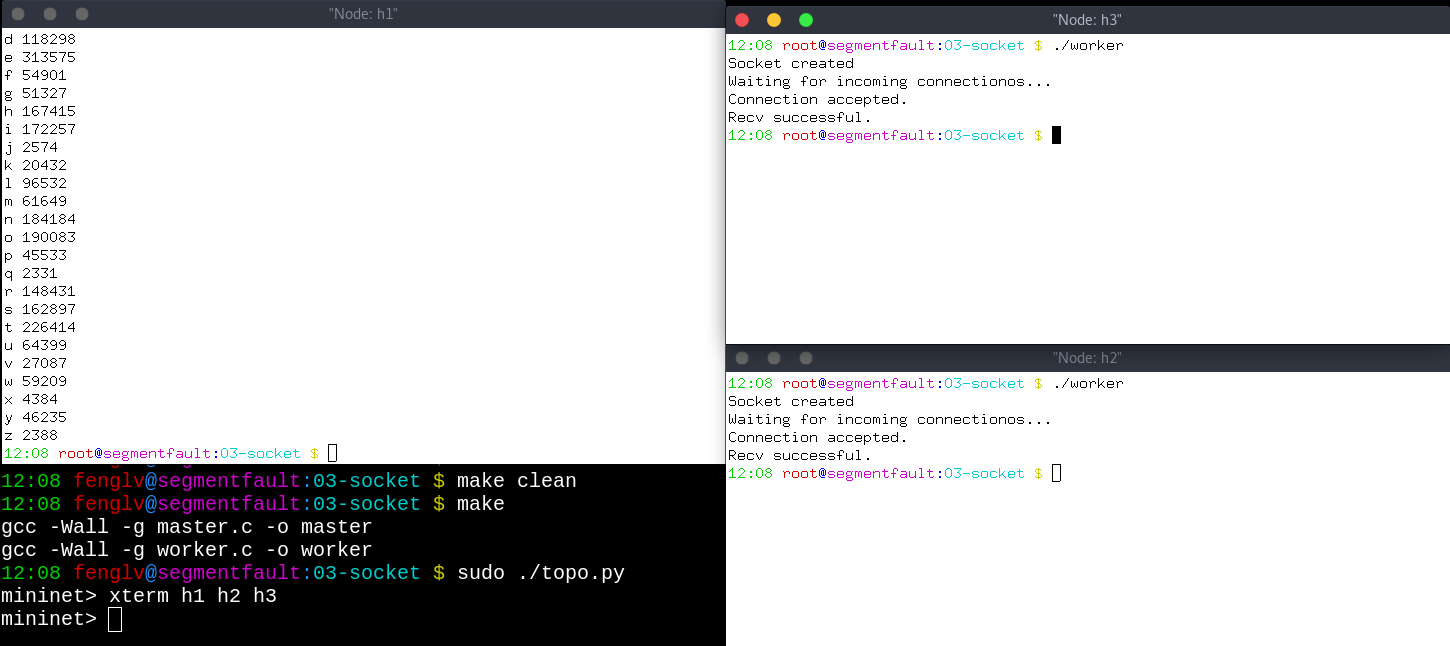
\includegraphics[scale = 0.3]{./sshot.png}
			\caption{$Socket$应用编程实验运行截图}
			\end{figure}
		%\hline
		\section*{{\CJKfamily{zhhei}结果分析}}在刚开始,由于一些内存错误,导致$worker$运行时出现$segmentation\ fault$,后经过调试,程序能够按照实验要求正确运行,输出结果与$reference$程序一样。\\
			%\hline
			%  \end{tabular}
			%\end{center}
			\end{document}


